\chapter{Fundamentação Teórica}
\label{cap:fundamentacao-teorica}

Neste capítulo, serão explorados os fundamentos teóricos essenciais relacionados à compressão de dados, um campo vital na ciência da computação e na transmissão eficiente de informações. Abordamos os dois principais paradigmas de compressão, com perda e sem perda, discutindo os princípios subjacentes, as aplicações relevantes e as métricas comumente usadas para avaliar a eficácia de cada abordagem. Esses conceitos fundamentais são essenciais para compreender em detalhes os algoritmos específicos de compressão e sua aplicação no contexto prático de otimização de imagens médicas.

\section{Compressão de Dados}
\label{sec:compressão-de-dados}
A compressão de dados é um campo essencial na área da tecnologia da informação que visa reduzir o espaço de armazenamento e a largura de banda necessária para transmissão de informações sem comprometer a integridade dos dados. A Figura~\ref{fig:compression-example} ilustra a comparação de tamanho entre uma imagem original e uma imagem comprimida. O primeiro contato  significativo com a compressão de dados foi com a codificação de Huffman em 1952 \cite{huffmanArticle}, marco fundamental que estabeleceu as bases teóricas para a eficiente representação de informações.

\begin{figure}[!htbp]
	\centering
	\UNIFORfig{
	    \Caption{\label{fig:compression-example} Exemplo de compressão de imagem.}
	}{
	    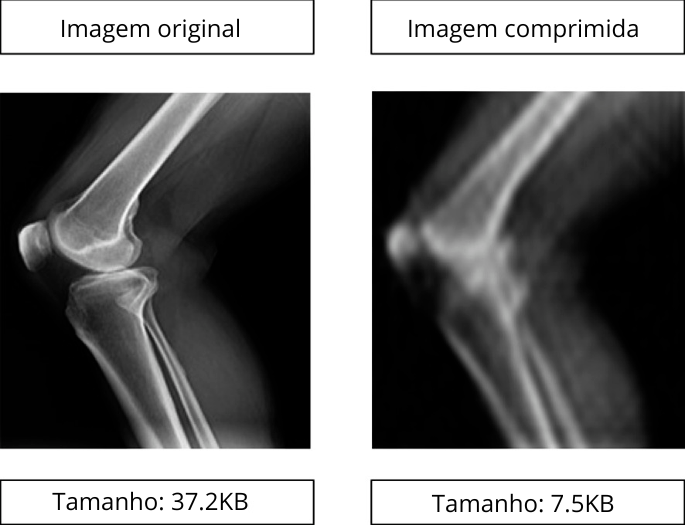
\includegraphics[width=0.55\textwidth]{images/compression-example.png}
	}{
	    \Fonte{Adaptada de \cite{imageCompressionExample}}
	}	
\end{figure}

\subsection{Taxa de compressão}
A taxa de compressão, ou do inglês \acrfull{CR}, é uma métrica crucial que quantifica a eficiência do processo de compressão. Ela é definida como a razão entre o tamanho do arquivo comprimido (\(S_{\text{comprimido}})\) e o tamanho do arquivo original (\(S_{\text{original}})\):
\begin{center}
    \(\displaystyle CR = 1 - \frac{S_{\text{comprimido}}}{S_{\text{original}}}\)
\end{center} 

\noindent A Figura~\ref{fig:compression-ratio-example} ilustra um exemplo dessa taxa de compressão, no qual é possível perceber que, à medida que a taxa de compressão aumenta, o tamanho do arquivo diminui, resultando em perdas progressivas de qualidade da imagem. Grosso modo isso se da pois quanto mais detalhes uma imagem tem, mais bits são necessários para representar aquela imagem. Isso é evidente na comparação visual entre a imagem original e suas versões comprimidas.

\begin{figure}[!htbp]
	\centering
	\UNIFORfig{
	    \Caption{\label{fig:compression-ratio-example} Comparação entre diferentes taxas de compressão}
	}{
	    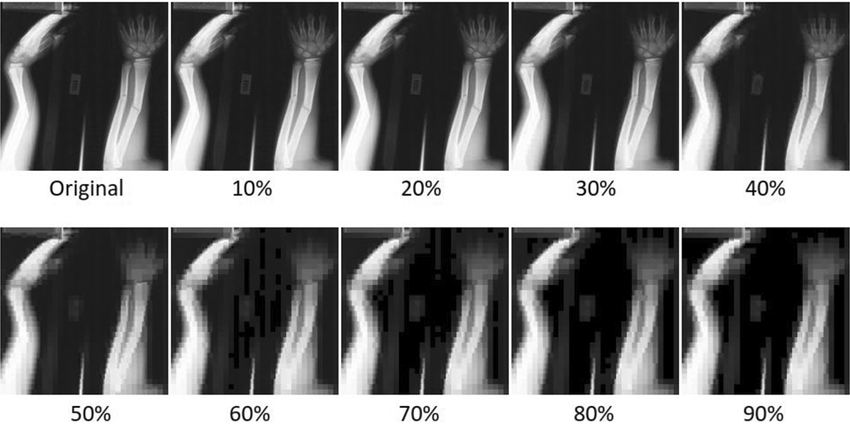
\includegraphics[width=\textwidth]{images/compression-ratio-example.png}
	}{
	    \Fonte{\cite{imageCompressionRate}}
	}	
\end{figure}
Quando falamos de compressão de dados, temos duas abordagens de algoritmos, os com perda e os sem perda, como ilustra a Figura~\ref{fig:lossless-vs-lossy}.

\begin{figure}[!htbp]
	\centering
	\UNIFORfig{
	    \Caption{\label{fig:lossless-vs-lossy} Comparação entre compressão com e sem perda}
	}{
	    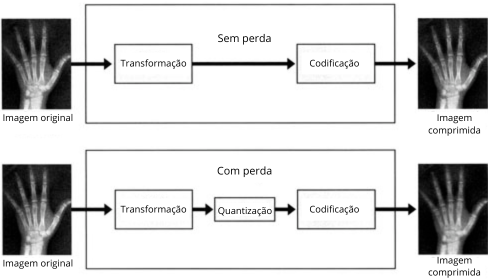
\includegraphics[width=\textwidth]{images/lossy-vs-lossless.png}
	}{
	    \Fonte{Adaptada de \cite{imageLossyVsLossless}}
	}	
\end{figure}

\subsection{Compressão sem perda}
A compressão sem perda preserva totalmente a informação original, explorando apenas a redundância dos dados e garantindo que a descompressão resulte no arquivo idêntico ao original. O algoritmo de Huffman \cite{huffmanArticle} é um exemplo clássico que utiliza códigos de comprimento variável para representar dados com diferentes frequências de ocorrência. Em outras palavras, em vez de atribuir um número fixo de bits para cada símbolo (como é o caso dos códigos de comprimento fixo), os códigos de comprimento variável permitem que símbolos mais comuns sejam representados por sequências de bits mais curtas, enquanto símbolos menos frequentes são representados por sequências de bits mais longas \cite{compressionTechniquesElakkiya}. Isso resulta em uma representação mais eficiente dos dados, uma vez que os símbolos mais comuns são codificados com menos bits, enquanto ainda mantém a capacidade de recuperar integralmente as informações originais durante o processo de descompressão. Essa abordagem de compressão é preferível em cenários em que nenhuma perda de integridade do documento é aceitável, como aqueles que envolvem documentos legais ou arquivos executáveis.

\subsection{Compressão com perda}
A compressão com perda, por outro lado, sacrifica parte da informação para obter uma maior taxa de compressão. Essa técnica é frequentemente empregada quando uma perda mínima de qualidade é aceitável para reduzir significativamente o tamanho do arquivo. Um exemplo comum é a compressão \acrshort{JPEG}. Ao contrário da compressão sem perda, que preserva integralmente as informações, a compressão com perda é mais flexível em relação à perda de informações. Ela é amplamente utilizada em cenários onde a qualidade ligeiramente inferior é aceitável em troca de uma redução significativa no tamanho do arquivo. Isso inclui aplicações como \textit{streaming} de vídeo, videoconferência e armazenamento de fotos em \textit{smartphones}. Para medir a perda resultante dessa compressão, uma métrica comumente empregada é o \acrfull{MSE}, que quantifica a diferença entre os valores originais e os valores comprimidos \cite{compressionTechniquesElakkiya}. A fórmula do \acrshort{MSE} é dada por:
\begin{center}
    \(\displaystyle MSE = \frac{\sum_{i=1}^{n} (X_i - Y_i)^2}{n}\)
\end{center}
\BlankLine
\noindent onde $n$ representa o número total de símbolos ou dados a serem comprimidos. A expressão \( \sum_{i=1}^{n} \) denota a soma dos termos, em que cada termo, $(X_i - Y_i)^2$, corresponde à diferença ao quadrado entre o valor original $X_i$ e o valor reconstruído $Y_i$ após a compressão. Essa operação garante que todas as diferenças sejam positivas e destaca as discrepâncias maiores entre os valores originais e os valores reconstruídos.

Além do \acrshort{MSE}, outra métrica comum para avaliar a perda de informações durante a compressão é a \acrfull{PSNR}. A \acrshort{PSNR} é frequentemente utilizada para medir a qualidade percebida da imagem após a compressão, fornecendo uma avaliação mais intuitiva para os usuários. A fórmula da \acrshort{PSNR} é dada por \cite{compressionTechniquesElakkiya}:
\begin{center}
    \(\displaystyle PSNR = 10 \cdot \log_{10}\left(\frac{\text{Valor Máximo}^2}{\text{MSE}}\right)\)
\end{center}
\BlankLine
Aqui, o Valor Máximo representa o maior valor possível de um pixel, geralmente representado pelo valor máximo que pode ser representado na imagem. Uma PSNR mais alta indica uma menor perda de informações e uma qualidade visual mais preservada. Essas métricas, como \acrshort{MSE} e \acrshort{PSNR}, fornecem maneiras objetivas de quantificar a perda de qualidade durante a compressão de dados, sendo ferramentas essenciais na avaliação do desempenho de algoritmos de compressão com perda.

\subsection{Entropia}
No contexto de compressão de imagem, a entropia é uma medida estatística que se refere à incerteza ou aleatoriedade das informações contidas em uma imagem. Quanto maior a entropia, mais imprevisíveis são os dados e mais difícil é comprimi-los. A entropia é frequentemente utilizada para  avaliar a eficiência da compressão sem perda, já que uma alta entropia implica em menor redundância nos dados, o que pode limitar a capacidade de compressão. A entropia de um conjunto de dados é calculada usando a teoria da informação de Shannon \cite{dataCopressionSayood}, sendo definida como a média ponderada das probabilidades dos símbolos no conjunto de dados. Matematicamente, a entropia de Shannon em bits $H(X)$ de uma variável aleatória discreta $X$ com distribuição de probabilidade $P(X)$ é definida por:
\BlankLine
\begin{center}
    \(\displaystyle H(X) = - \sum_{i=1}^{n} p(x_i) \log_2 p(x_i)\)
\end{center}

\noindent Onde $p(x_i)$ é a probabilidade do símbolo $(x_i)$ ocorrer no conjunto de dados.

Em imagens, a entropia é uma medida de quantidade de informação contida na imagem. Imagens com alta entropia tem uma maior variedade de cores e textura, o que torna mais difícil encontrar padrões repetidos e redundâncias que podem ser explorados para compressão, enquanto que imagens com baixa entropia têm menos variação e podem ser mais facilmente comprimidas. 

\subsection{\acrfull{DCT}}
A \acrfull{DCT} é uma técnica essencial na compressão de imagens, particularmente em algoritmos como o \acrshort{JPEG}. Ela desempenha um papel crucial ao converter os dados espaciais, ou seja, as informações sobre  a intensidade luminosa de cada pixel e sua localização na imagem em dados de frequência. Essa transformação é realizada por meio de uma série de operações matemáticas que convertem a informação de pixel em componentes de frequência \cite{digitalImageProcessingGonzalez}.

A \acrshort{DCT} divide a imagem em pequenos blocos e é aplicada a cada bloco separadamente. Durante esse processo, os padrões de variação são analisados na intensidade dos pixels dentro de cada bloco e são expressos em termos de frequência. Isso significa que a transformada identifica quais frequências estão presentes na imagem e em que intensidade, onde coeficientes de frequência de alta amplitude representam componentes de imagem que contribuem significativamente para a aparência visual, enquanto coeficientes de baixa amplitude representam detalhes menos perceptíveis. A definição da \acrshort{DCT} é dada por \cite{digitalImageProcessingGonzalez}:
\BlankLine
\begin{center}
    \(\displaystyle F(u,v) = \frac{1}{\sqrt{2N}}C(u)C(v)\sum_{x=0}^{N-1}\sum_{y=0}^{N-1}f(x,y)\cos\left[\frac{(2x + 1)u\pi}{2N}\right]\cos\left[\frac{(2y + 1)v\pi}{2N}\right]\)
\end{center}
\noindent onde $F(u,v)$ é o coeficiente da transformada na posição $(u,v)$, $f(x,y)$ é o valor do pixel na posição $(x,y)$, $N$ é o tamanho da imagem $C(u)$ e $C(v)$ são coeficientes de normalização. A expressão matemática da \acrshort{DCT} descreve como a transformação é realizada mapeando os valores de intensidade dos pixels para coeficientes de frequência, concentrando a energia da imagem nos coeficientes  de frequência mais significativos e descartando ou reduzindo os coeficientes de frequência de baixa amplitude

\subsection{Quantização}
A quantização é uma etapa essencial da compressão de imagem, que depende diretamente da \acrshort{DCT}. Após a aplicação da \acrshort{DCT}, os coeficientes de frequência resultantes são quantizados para reduzir a quantidade de dados necessários para representar a imagem. Esta etapa é critica, pois determina o nível de perda de qualidade que ocorrerá na imagem comprimida. A quantização é realizada dividindo-se os coeficientes de frequência pelos valores correspondentes na matriz de quantização e arredondando os resultados para o valor mais próximo. Isso resulta na perda de informações menos importantes da imagem, o que leva a uma redução significativa no tamanho da imagem \cite{quantizationGersho}.

A matriz de quantização controla o nível de compressão e, consequentemente, a taxa de perda de qualidade. Ao ajustar os valores na matriz de quantização, é possível parametrizar a compressão para comprimir mais ou menos. Reduzir os  valores na matriz de quantização resulta em uma compressão mais agressiva, o que leva a uma maior perda de qualidade na imagem comprimida. Por outro lado, aumentar os valores na matriz de quantização produz uma compressão menos agressiva, preservando mais detalhes na imagem. A quantização é definida por: 
\BlankLine
\begin{center}
    \(\displaystyle F_q(u,v) = \text{round}\left(\frac{F(u,v)}{Q(u,v)}\right) \)
\end{center}

\noindent Onde \textit{\(F_q\)(u,v)} é o coeficiente de frequência quantizado, $F(u,v)$ é o coeficiente de frequência original obtido pela \acrshort{DCT}, e $Q(u,v)$ é o valor correspondente na matriz de quantização. Essa equação exemplifica como a quantização é realizada, ajustando os coeficientes de frequência para reduzir a quantidade necessária de dados para  representar a imagem \cite{quantizationGersho}. A Figura~\ref{fig:quantization-example} compara três diferentes níveis de quantização, demonstrando como o aumento da quantização, ou seja, a diminuição de dados necessários para representar a imagem, afeta a nitidez, os detalhes e a fidelidade visual da imagem comprimida. 

\begin{figure}[H]
	\centering
	\UNIFORfig{
	    \Caption{\label{fig:quantization-example} Comparação entre diferentes níveis de quantização}
	}{
	    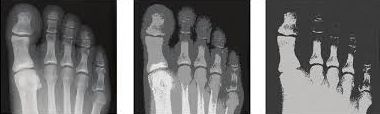
\includegraphics[width=\textwidth]{images/quantization-example.png}
	}{
	    \Fonte{Adaptada de \cite{imageQuantization}}
	}	
\end{figure}

\subsection{\acrfull{RGB} vs Escala de cinza (Grayscale)}
Imagens em \acrfull{RGB} são compostas por três canais de cores: vermelho, verde e azul. Cada pixel na imagem é representado por uma combinação desses três canais, onde a intensidade de cada canal determina a cor específica desse pixel. Geralmente, cada canal é representado por 8 bits, o que significa que cada canal pode ter 256 valores diferentes de intensidade, variando de 0 a 255. Portanto, uma imagem RGB típica possui 24 bits, ou 3 bytes, por pixel (8 bits para cada canal), resultando em uma gama de cores muito ampla e uma representação rica da imagem \cite{digitalImageProcessingGonzalez}.

Por outro lado, as imagens em escala de cinza são compostas por apenas um canal de intensidade luminosa, onde a cor de cada pixel é representada por um único valor de intensidade. Cada pixel em uma imagem em escala de cinza é representado por um valor de 8 bits, variando de 0 a 255, onde 0 representa preto e 255 representa branco \cite{digitalImageProcessingGonzalez}. Essa representação simplificada é adequada para imagens médicas, como as tomografias, onde a ênfase está na intensidade do sinal em vez das cores.

As imagens em escala de cinza requerem menos espaço de armazenamento e processamento computacional em comparação com as imagens RGB, o que é vantajoso ao lidar com grandes conjuntos de dados de tomografia. Portanto, ao analisar imagens de tomografia, é comum utilizar imagens em escala de cinza para representar com precisão as informações médicas relevantes.

\begin{figure}[H]
	\centering
	\UNIFORfig{
	    \Caption{\label{fig:rgb-grayscale-example} Visualização de uma imagem em escala de cinza e \acrshort{RGB}}
	}{
	    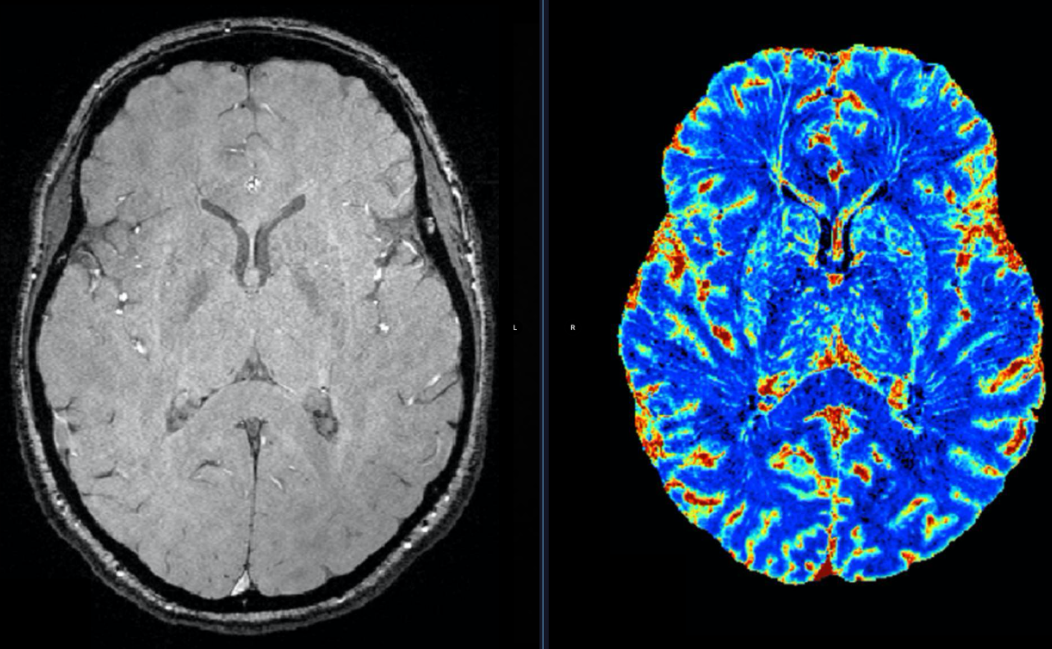
\includegraphics[width=\textwidth]{images/rgb-grayscale-example.png}
	}{
	    \Fonte{Extraída de \cite{imageRgbGrayscale}}
	}	
\end{figure}


\section{\acrfull{DICOM}}
O \acrshort{DICOM} é um padrão internacional fundamental para o armazenamento, transmissão e troca de informação de imagens médicas digitais \cite{DICOM}. Além de fornecer um formato padronizado, o \acrshort{DICOM} também estabelece diretrizes para metadados associados, como informações de paciente, estudo, série e imagem, como ilustrado na Figura~\ref{fig:dicom-metadata}. Uma característica distintiva das imagens \acrshort{DICOM} é a inclusão desses metadados detalhados, que permitem uma melhor compreensão e interpretação das imagens no contexto clínico.

Uma imagem é considerada \acrshort{DICOM} quando segue as especificações do padrão \acrshort{DICOM}, incluindo a estrutura de metadados e os requisitos de formato de arquivo. Essas imagens podem ser adquiridas por uma variedade de dispositivos médicos, como tomógrafos, ressonâncias magnéticas e sistemas de ultrassom, e são comumente usadas em diagnósticos por imagem, planejamento de tratamento e monitoramento de pacientes.

Quanto à compressão, as imagens \acrshort{DICOM} podem ser armazenadas em formato comprimido ou não comprimido, e essa informação é incluída nos metadados da imagem através do atributo \textit{TransferSyntaxUID}, onde este indica o esquema de codificação ou compressão de dados aplicado a uma imagem ou conjunto de dados \acrshort{DICOM}, e a ausência desse campo indica que a imagem não está comprimida \cite{DICOM}.

Embora seja amplamente adotado, ele tende a gerar arquivos volumosos devido aos metadados detalhados. Isso representa um desafio para o armazenamento eficiente, especialmente em ambientes hospitalares. A compressão de imagens \acrshort{DICOM} é uma solução, mas pode impactar na qualidade diagnóstica, especialmente com compressão com perda. É essencial encontrar um equilíbrio entre a redução do tamanho dos arquivos e a preservação da qualidade das imagens para garantir diagnósticos precisos e tratamentos eficazes na prática clínica. A Figura~\ref{fig:dicom-example} ilustra a visualização de uma imagem \acrshort{DICOM}.

\begin{figure}[H]
	\centering
	\UNIFORfig{
	    \Caption{\label{fig:dicom-metadata} Metadados de uma imagem \acrshort{DICOM}}
	}{
	    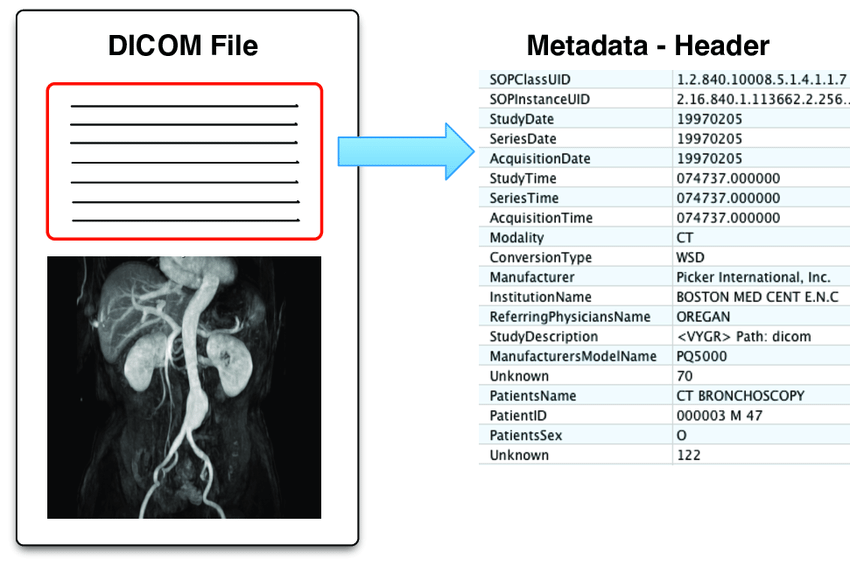
\includegraphics[width=\textwidth]{images/dicom-metadata.png}
	}{
	    \Fonte{Extraída de \cite{imageDicomMetadata}}
	}	
\end{figure}

\begin{figure}[H]
	\centering
	\UNIFORfig{
	    \Caption{\label{fig:dicom-example} Visualização de uma imagem \acrshort{DICOM}}
	}{
	    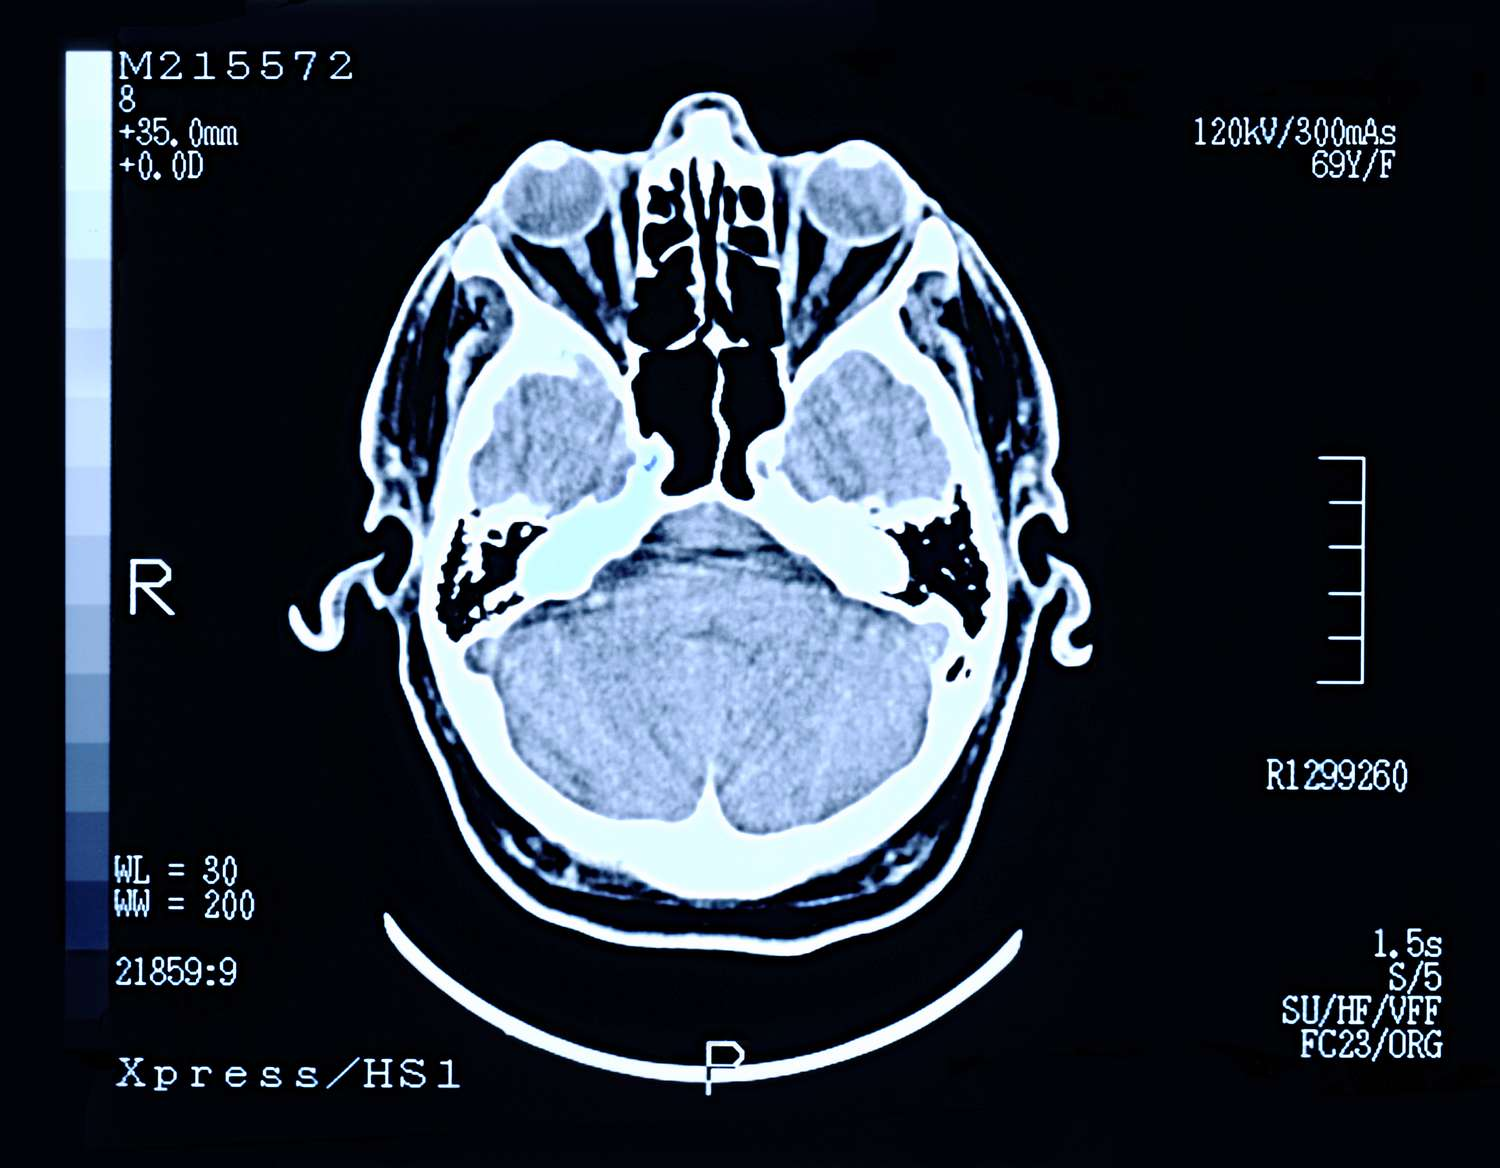
\includegraphics[width=\textwidth]{images/dicom-example.jpg}
	}{
	    \Fonte{Extraída de \cite{imageDicom}}
	}	
\end{figure}

\section{Algoritmo de Huffman}
O algoritmo de Huffman \cite{huffmanArticle} é um método de compressão sem perda que utiliza codificação de comprimento variável para representar símbolos de entrada com base em suas frequências de ocorrência. Desenvolvido em 1952 por David A. Huffman, esse algoritmo tem sido amplamente utilizado em uma variedade de aplicações de compressão de dados.

\begin{figure}[!htbp]
    \centering
    \UNIFORfig{
        \Caption{\label{fig:huffman-coding} Árvore de Huffman para uma sequência de caracteres aleatórios}
    }{
        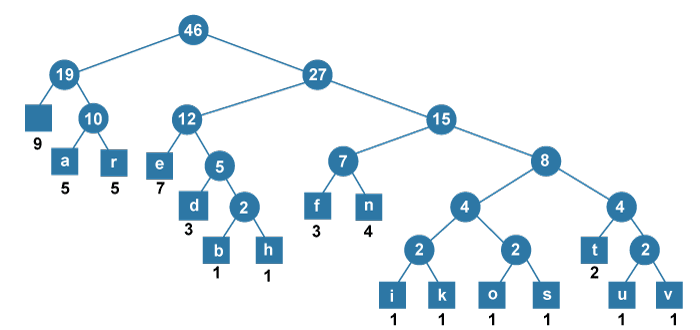
\includegraphics[width=\textwidth]{images/huffman-coding.png}
    }{
        \Fonte{\cite{imageHuffmanTree}}
    }   
\end{figure}

Para fins de ilustração, na Figura~\ref{fig:huffman-coding}, podemos ver que o símbolo ``a'' possui 5 ocorrências, enquanto o símbolo ``v'' possui apenas uma, então o caminho (quantidade de bits) para se representar o ``a'' é menor do que para se representar o ``v''.

O processo de compressão consiste nas seguintes etapas:
\begin{enumerate}
    \item Leitura dos dados de entrada:
    \BlankLine
    Todo o conteúdo do arquivo é lido do disco e armazenado na memória para manipulação posterior. Este passo é estratégico para o desempenho do algoritmo, pois permite que os dados sejam processados de forma eficiente. Uma abordagem alternativa seria processar os dados diretamente no arquivo, mas isso poderia resultar em perda de desempenho, especialmente para arquivos muito grandes.
    
    \item Construção da Fila de Prioridade:
    \BlankLine
    Nesta etapa do algoritmo de Huffman, os dados são utilizados para criar uma fila de prioridade com base na frequência de ocorrência dos símbolos presentes no texto original. Essa fila de prioridade é uma estrutura de dados que organiza os elementos de acordo com sua relevância, garantindo que os símbolos mais frequentes, que tendem a ter códigos mais curtos, sejam processados primeiro durante a construção da árvore de Huffman. Cada vez que um novo símbolo é encontrado no texto original, um nó é criado na fila de prioridade. Se o símbolo já está presente na fila, sua frequência é incrementada e o nó correspondente é reordenado na lista.

    \item Construção da Árvore Trie:
    \BlankLine
    A partir da fila de prioridade construída anteriormente, os dois nós de menor frequência (os dois primeiros) são removidos da fila e combinados para formar um novo nó que é reinserido na fila. Esse processo é repetido até que apenas um nó permaneça na fila, representando a raiz da árvore de Huffman. Esta árvore é ilustrada na Figura~\ref{fig:huffman-coding}.

    \item Construção da Tabela de Códigos:
    \BlankLine
    Uma vez construída a árvore de Huffman, uma tabela de códigos é criada para mapear cada símbolo ao seu código binário correspondente. Isso é feito percorrendo a árvore recursivamente, atribuindo códigos binários aos símbolos folha \cite{imeUspBinaryTrees}. Os símbolos mais frequentes recebem códigos mais curtos, enquanto os menos frequentes recebem códigos mais longos.

    \item Transformação do texto original em cadeia de bits:
    \BlankLine
    Utilizando a tabela de códigos, o texto original é transformado em uma cadeia de bits substituindo cada símbolo pelo seu código correspondente. Isso resulta em uma representação compacta do texto original, composta apenas por zeros e uns.

    \item Construção do fluxo de bytes comprimidos:
    \BlankLine
    A cadeia de bits gerada na etapa anterior é convertida em um fluxo de bytes comprimido, necessário porque os dados são armazenados em arquivos binários, e não diretamente como bits individuais.
\end{enumerate}

Uma das principais vantagens do algoritmo de Huffman \cite{huffmanArticle} é a sua capacidade de produzir uma representação compacta dos dados, especialmente para conjuntos de dados com distribuições de frequência desiguais. No entanto, a eficiência do algoritmo depende da capacidade de prever as frequências de ocorrência dos símbolos de entrada com precisão. Em alguns casos, a construção da árvore de Huffman pode ser computacionalmente intensiva, especialmente para conjuntos de dados grandes \cite{huffmanArticle}.

A complexidade de espaço do algoritmo de Huffman é dominada pelo tamanho da árvore de Huffman e pela tabela de códigos resultante, aproximadamente \( O(n) \) para uma árvore ótima, onde \( n \) é o número de símbolos distintos na entrada. Em termos de tempo, a construção da árvore de Huffman é \( O(n \log n) \) devido à combinação na fila de prioridade, enquanto a compressão dos dados é \( O(m) \), com \( m \) sendo o número total de bits no texto original. Essas características tornam o algoritmo de Huffman eficiente para compressão de dados em várias aplicações.

\begin{algorithm}[H]
\SetAlgoLined
\DontPrintSemicolon

\KwIn{Conjunto de caracteres e suas frequências}
\KwOut{Tabela de códigos de Huffman}

\BlankLine
Inicializar uma fila de prioridade $Q$ com os nós folha para cada caractere com sua frequência;
\While{$|Q| > 1$}{
$x \gets$ extrair o nó de menor frequência de $Q$;
\BlankLine
$y \gets$ extrair o próximo nó de menor frequência de $Q$;
\BlankLine
Criar um novo nó $z$ como nó interno com frequência $freq(z) = freq(x) + freq(y)$;
\BlankLine
$z$.esquerda $\gets x$;
\BlankLine
$z$.direita $\gets y$;
\BlankLine
Inserir $z$ de volta em $Q$;
}
Árvore de Huffman resultante é a única raiz restante em $Q$;
Derivar os códigos de Huffman percorrendo a árvore a partir da raiz;

\caption{Codificação de Huffman}
\end{algorithm}

\section{Algoritmos de compressão de imagens}
\subsection{\acrfull{PNG}}
\acrshort{PNG} é um formato de arquivo de imagem amplamente difundido que utiliza compressão sem perda de dados. A compressão \acrshort{PNG} é baseada no algoritmo DEFLATE \cite{dataCopressionSayood}, que é uma combinação de  dois outros algoritmos: \acrfull{LZ77} \cite{lempelZivArticle} e Huffman \cite{huffmanArticle}.
O processo de compressão de uma imagem para o formato \acrshort{PNG} consiste nas seguinte etapas:
\begin{enumerate}
    \item Pré-processamento:
    \BlankLine
    Antes da compressão, a imagem passa por um pré-processamento que pode incluir técnicas como o \textit{filtering prediction} \cite{compressionTechniquesElakkiya}. O \textit{filtering prediction} aplica filtros preditivos aos dados de imagem para estimar os valores dos pixels com base nos valores dos pixels vizinhos, ou seja, aqueles que estão na mesma linha ou coluna \cite{compressionTechniquesElakkiya}. Existem cinco tipos de filtros preditivos utilizados no formato PNG:
    \begin{itemize}
        \item Nenhum: Sem filtragem, os valores dos pixels são usados diretamente.
        \item Sub: O valor do pixel atual menos o valor do pixel anterior na linha.
        \item Up: O valor do pixel atual menos o valor do pixel acima na coluna.
        \item Average: A média dos pixels anterior na linha e acima na coluna subtraída do valor do pixel atual.
        \item Paeth: Um algoritmo que usa uma função preditiva para escolher o pixel mais próximo entre os pixels anterior, acima e a soma dos dois menos o pixel na diagonal superior esquerda.
    \end{itemize}
    O filtro de predição por subtração, por exemplo, pode ser representado pela seguinte fórmula:
    \begin{center}
        \(\displaystyle Pixel_{\text{predito}} = Pixel_{\text{atual}} - Pixel_{\text{vizinho}}\)
    \end{center}
    Ao aplicar esses filtros, a redundância nos dados de imagem é reduzida, o que aumenta a eficiência do algoritmo de compressão DEFLATE. Isso resulta em arquivos \acrshort{PNG} mais compactos e mais eficientes para armazenamento.

    \item Compressão com DEFLATE:
    \BlankLine
    O DEFLATE opera em duas principais etapas: a compactação com \acrshort{LZ77} e codificação de Huffman
    \begin{itemize}
        \item Compactação:
        O algoritmo \acrshort{LZ77} \cite{lempelZivArticle} procura por padrões repetidos de dados dentro de bloco. Ele substitui esses padrões por referências a cópias anteriores dos mesmos dados, seguido pela distância e pelo comprimento dessas cópias. Isso reduz a redundância nos dados e permite uma representação mais compacta.

        \item Codificação:
        Após a compactação, os dados da imagem são codificados usando o algoritmo de codificação de Huffman \cite{huffmanArticle}. Este atribui códigos mais curtos para padrões de pixels comuns, enquanto símbolos menos comuns, como detalhes finos ou ruído de imagem, recebem  códigos mais longos, resultando em uma representação mais eficiente, onde a informação visual é preservada de forma otimizada.
    \end{itemize}

    \item Estruturação em Chunks:
    \BlankLine
    A imagem \acrshort{PNG} é organizada em pedaços chamados "chunks". Cada chunk contém uma parte específica dos dados da imagem ou metadados. Os principais chunks incluem:

    \begin{itemize}
        \item IHDR: Contém informações básicas da imagem, como largura, altura, profundidade de cor e tipo de cor.
        \item IDAT: Contém os dados da imagem comprimidos.
        \item PLTE: Contém a paleta de cores, se aplicável.
        \item IEND: Indica o fim da imagem.
    \end{itemize}
    
\end{enumerate}
\BlankLine

\noindent As etapas de compressão do \acrshort{PNG}, como o pré-processamento, compressão com DEFLATE, e estruturação em chunks, são essenciais para reduzir o tamanho dos arquivos de imagem mantendo sua qualidade. \textit{filtering prediction} reduz a redundância, enquanto o DEFLATE proporciona uma compressão eficiente \cite{digitalImageProcessingGonzalez}. Essas etapas garantem arquivos compactos sem comprometer a qualidade da imagem.

\begin{figure}[!htbp]
	\centering
	\UNIFORfig{
	    \Caption{\label{fig:png-compression-example} Compressão de imagem com \acrshort{PNG}}
	}{
	    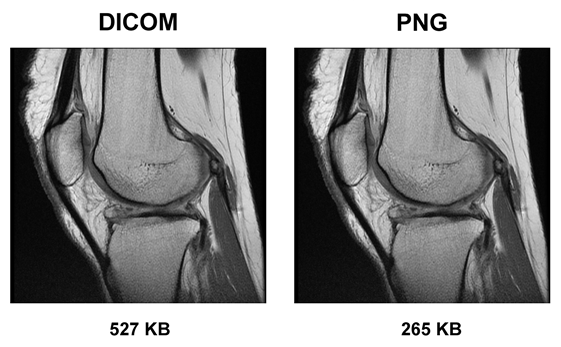
\includegraphics[width=\textwidth]{images/png-compression-example.png}
	}{
	    \Fonte{\cite{imagePNGCompression}}
	}	
\end{figure}

Considerando o desempenho da compressão \acrshort{PNG}, é crucial analisar tanto a complexidade de espaço quanto de tempo envolvida nesse processo. Em termos de complexidade de espaço, a quantidade de memória necessária para armazenar os dados intermediários durante a compressão e descompressão impacta diretamente no desempenho. Isso inclui a memória utilizada para manter as estruturas de dados para a fila de prioridade e a árvore de Huffman \cite{huffmanArticle}, bem como os \textit{buffers} para armazenar os dados comprimidos e descomprimidos. Além disso, a complexidade de tempo é influenciada pelo tamanho em bytes da imagem, uma vez que a aplicação dos algoritmos é realizada para a imagem inteira. Quanto maior o tamanho da imagem, mais tempo será necessário para processá-la. Todos esses fatores combinados podem impactar a complexidade de tempo e espaço da compressão \acrshort{PNG}. \cite{digitalImageProcessingGonzalez}


% JPG
\subsection{\acrfull{JPEG}}
\acrshort{JPEG} é um formato de compressão de imagens com perdas amplamente utilizado que emprega uma combinação de técnicas para reduzir o tamanho do arquivo, sem perder muita qualidade visual \cite{miano1999compressed}. Para imagens coloridas, o processo de compressão \acrshort{JPEG} envolve várias etapas fundamentais, incluindo a conversão de espaço de cores e \textit{downsampling}. No entanto, para imagens em escala de cinza, como elas possuem apenas um canal de cor (luminância) e não têm componentes de crominância, essas duas etapas não são necessárias \cite{digitalImageProcessingGonzalez}. Portanto, o processo de compressão \acrshort{JPEG} para imagens em escala  de cinza é simplificado em comparação com imagens coloridas. A Figura~\ref{fig:jpeg-flow} ilustra o processo de compressão e descompressão desse formato, as etapas principais incluem:

\begin{figure}[H]
	\centering
	\UNIFORfig{
	    \Caption{\label{fig:jpeg-flow} Fluxo de compressão e descompressão do \acrshort{JPEG}}
	}{
	    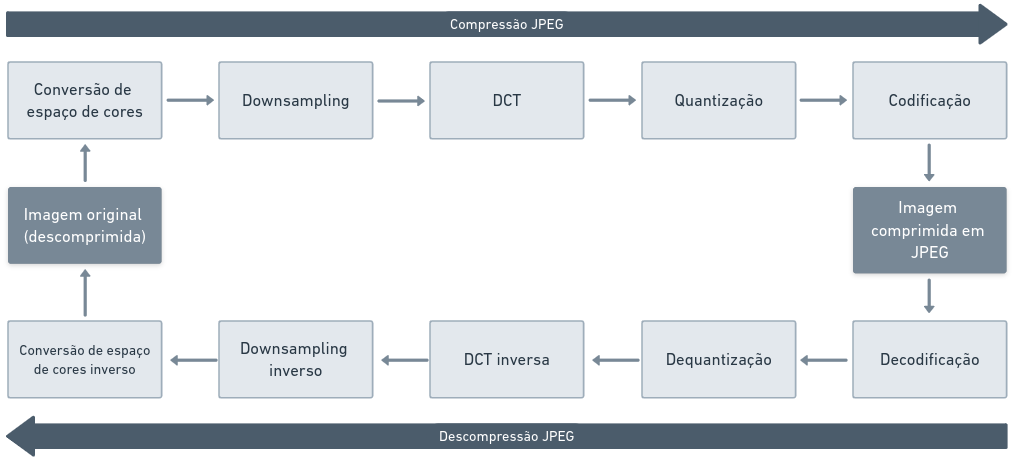
\includegraphics[width=\textwidth]{images/jpeg-flow.png}
	}{
	    \Fonte{Elaborado pelo autor}
	}	
\end{figure}

\begin{enumerate}
    \item Conversão de Espaço de Cores (\textit{Color Space Conversion}):
    Antes da compressão, a imagem é convertida de  seu espaço de cores original para outro espaço de cores mais adequado. Isso é especialmente importante para imagens em  escala de cinza, onde a conversão para um espaço de cores como o YCbCr pode melhorar a eficiência da compressão. No caso das imagens em escala de cinza, embora tenham apenas um canal de cor (luminância), a conversão para o espaço de cores YCbCr ainda pode ser benéfica. Isso ocorre porque a representação YCbCr separa a informação de luminância (Y) das informações de crominância (Cb e Cr), permitindo que a compressão se concentre principalmente na luminância, que é mais perceptível aos olhos humanos \cite{miano1999compressed}.

    \item \textit{Downsampling:}
    A etapa de \textit{downsampling} é usada para reduzir a resolução das componentes de crominância (Cb e Cr) mantendo a resolução da luminância (Y). Isso é feito porque as informações de cor nas imagens podem ser redundantes, especialmente nas componentes de crominância. No entanto, para imagens em escala de cinza, essa etapa é ignorada, pois não há informações de crominância para serem amostradas \cite{miano1999compressed}.

    \item \acrshort{DCT}:
    Após a conversão do espaço de cores e o \textit{downsampling}, cada bloco da imagem é submetido à transformada discreta do cosseno \acrshort{DCT}. Essa converte os dados espaciais da imagem em coeficientes de frequência, separando os componentes de alta e baixa frequência. Isso permite uma representação mais eficiente da imagem, concentrando a energia nos coeficientes de frequência mais significativos \cite{miano1999compressed}.

    \item Quantização:
    Os coeficientes de frequência resultantes da \acrshort{DCT} são quantizados para reduzir a quantidade de dados necessários para representar a imagem, Esta etapa introduz perda de qualidade, pois envolve a redução da precisão dos coeficientes de frequência menos significativos. A matriz de quantização é ajustada para controlar o nível de compressão e, consequentemente, a taxa de perda de qualidade \cite{miano1999compressed}.

    \item \textit{Run-Length Encoding} e \textit{Huffman Coding}:
    Após a quantização, os coeficientes de frequência quantizados são submetidos à codificação de \acrfull{RLE} e, em seguida, à codificação de Huffman \cite{huffmanArticle}. A codificação \acrshort{RLE} é utilizada para comprimir sequências de zeros consecutivos nos dados quantizados, enquanto a codificação de Huffman \cite{huffmanArticle} atribui códigos de comprimento variável aos símbolos com base em sua probabilidade de ocorrência. Essas técnicas de codificação contribuem para uma compressão eficiente dos dados, reduzindo ainda mais o tamanho da imagem \cite{miano1999compressed}.
\end{enumerate}

\noindent Essas etapas juntas compõem o processo de compressão \acrshort{JPEG}, que possibilita a redução do tamanho do arquivo de imagem com perdas controladas. Embora a qualidade da imagem seja comprometida devido à perda de informações durante a quantização, o algoritmo \acrshort{JPEG} oferece um equilíbrio adequado entre tamanho do arquivo e qualidade visual aceitável para uma ampla gama de aplicações \cite{digitalImageProcessingGonzalez}.

Considerando o desempenho da compressão \acrshort{JPEG}, é crucial analisar tanto a complexidade de espaço quanto de tempo envolvida nesse processo. Em termos de complexidade de espaço, a quantidade de memória necessária para armazenar os dados intermediários durante a compressão e descompressão impacta diretamente no desempenho. Isso inclui a memória utilizada para manter os blocos de pixels, as estruturas de dados para a fila de prioridade e as tabelas de Huffman, bem como os buffers para armazenar os dados comprimidos e descomprimidos. Além disso, a complexidade de tempo é influenciada pelo tamanho em bytes da imagem, uma vez que a compactação é realizada para cada bloco individualmente. Quanto maior o tamanho da imagem, mais blocos serão processados, aumentando assim a complexidade de tempo da compressão e descompressão \acrshort{JPEG}. Todos esses fatores combinados podem impactar a eficiência e o desempenho geral da compressão \acrshort{JPEG}.

\subsection{\acrfull{PCA}}
\acrfull{PCA} é uma técnica fundamental em análise de dados e  aprendizado de máquina amplamente utilizada para redução de dimensionalidade de dados \cite{multivariateAnalysis}. O \acrshort{PCA} é uma abordagem estatística que busca encontrar as direções de maior variabilidade nos dados, representadas pelos autovetores da matriz de covariância, e projetar os dados nesses componentes principais. Essa técnica tem aplicações em diversas áreas, incluindo reconhecimento de padrões, visão computacional e compressão de dados. As etapas principais dessa abordagem para compressão de imagens são:

\begin{enumerate}
    \item Preparação da imagem:
    A imagem é convertida para escala de cinza, reduzindo a quantidade de canais da imagem, mantendo apenas o canal de nível de cinza, sendo cada pixel representado por um valor entre 0 e 255, onde 0 é preto, e 255, branco \cite{multivariateAnalysis}.

    \item Organização dos dados:
    A matriz de pixels é convertida em um vetor unidimensional de tamanho $m \times n$, onde $m$ representa a quantidade  de linhas e $n$ a quantidade de colunas da matriz, ou seja, se a imagem tiver uma resolução de 512x512 o resultado seria um vetor unidimensional de tamanho 262.144 (512x512), onde cada elemento do vetor representa a intensidade do pixel em uma posição especifica da imagem \cite{multivariateAnalysis}.

    \item Centralização dos dados:
    Após a organização dos dados, é calculada a média de todos  os valores de intensidade dos pixels na imagem. O valor dessa média é subtraído de cada valor de pixel no vetor de dados. Isso centraliza  os dados em torno de zero, removendo a informação de brilho médio da imagem \cite{multivariateAnalysis}.

    \item Cálculo da matriz de covariância:
    A partir da centralização dos dados, é calculada a matriz de covariância. Covariância entre dois pixels indica como eles variam juntos, uma covariância positiva entre os pixels sugere que eles variam juntos na mesma direção, enquanto uma covariância negativa indica que eles variam em direções opostas. Isso ajuda a identificar as direções principais de variabilidade nos dados, que são representadas pelos autovetores da matriz de covariância. Essas direções principais são usadas para comprimir e reconstruir a imagem com perda mínima de informação \cite{multivariateAnalysis}.

    \item Decomposição da matriz  de covariância:
    Decompondo a matriz de covariância são obtidos os autovetores e autovalores. Onde os autovetores representam as direções principais de variabilidade nos dados, enquanto os autovalores indicam a quantidade de variância ao longo de cada uma dessas direções \cite{multivariateAnalysis}.

    \item Seleção dos componentes principais:
    Após a decomposição da matriz de covariância, os autovetores são ordenados de acordo com seus autovalores correspondentes, em ordem decrescente. Dessa forma, os autovetores com os maiores autovalores contêm a maior parte da variância dos dados e, portanto, são tratados como os componentes principais \cite{multivariateAnalysis}.

    \item Compressão:
    Nesta etapa, o algoritmo se torna parametrizável, permitindo que escolhamos a quantidade de componentes principais para representar a imagem. Em outras palavras, quanto menos componentes principais forem selecionados, maior será a taxa de compressão e menor será a qualidade da imagem resultante. Ao escolher a quantidade de componentes principais, é multiplicado o  vetor de dados centralizados pelos autovetores correspondentes aos $n$ maiores autovalores, onde $n$ é o número de componentes selecionados, e então é adicionado a média de volta ao vetor resultante. Isso constrói uma versão comprimida da imagem original em formato de vetor, mantendo apenas as informações mais relevantes em termos de  variabilidade de dados \cite{multivariateAnalysis}.

    \item Descompressão:
    Para reconstruir a imagem original, é multiplicada o vetor comprimido da imagem original pelos autovetores transpostos (ou seja, os autovetores originais), e então adicionada a média de volta para obter a imagem reconstruída \cite{multivariateAnalysis}.
    
\end{enumerate}